% There are several document classes available
% For longer documents, you can use
% book or report
\documentclass[a4paper]{article} 
\usepackage{graphicx}
\usepackage{amsmath}
\usepackage{amssymb}
\usepackage{amsthm}
\usepackage{mathtools}
\usepackage{biblatex} %Imports biblatex package
\usepackage{subfig}
\usepackage{parskip}
\usepackage{multirow}
\usepackage{longtable}
\usepackage{booktabs}
\usepackage[most]{tcolorbox}
\usepackage{xcolor}
\addbibresource{stg3a.bib} %Import the bibliography file
\bibliography{stg3a}
\usepackage[hidelinks,colorlinks=true,linkcolor=blue,citecolor=red,urlcolor=blue]{hyperref}

% You can change the parameters: here are the available options:
% - a4paper
% - fancysections
% - notitlepage or titlepage
% - onside or twoside depending on whether you want to print double-sided or single-sided
% - sectionmark
% - chaptermark (for 
% - pagenumber
% - enmanquedinspiration
% In case of doubts, the documentation is at:
%  https://gitlab.binets.fr/typographix/polytechnique/-/blob/master/source/polytechnique.pdf



\usepackage[a4paper,  fancysections,  titlepage]{polytechnique}
\usepackage[english]{babel}
\usepackage[T1]{fontenc}
\usepackage{blindtext}
\usepackage[hidelinks]{hyperref}

\usepackage{listings}
\usepackage{tikz}
\usetikzlibrary{positioning,shadows}
\usepackage{xcolor}
\lstset{
  language=Python,
  basicstyle=\ttfamily\small,
  breaklines=true,
  showstringspaces = false,
  keywordstyle=\color{blue},
  stringstyle=\color{red},
  commentstyle=\color{brown},
  morecomment=[l][\color{magenta}]{\#},
  inputencoding=utf8,
  extendedchars=true,
  literate={à}{{\`a}}1 {ç}{{\c{c}}}1 {é}{{\'e}}1 {è}{{\`e}}1 {ê}{{\^e}}1 {ë}{{\"e}}1 {î}{{\^i}}1 {ï}{{\"i}}1 {ô}{{\^o}}1 {ö}{{\"o}}1 {ù}{{\`u}}1 {û}{{\^u}}1 {ü}{{\"u}}1 {ÿ}{{\"y}}1 {À}{{\`A}}1 {Ç}{{\c{C}}}1 {É}{{\'E}}1 {È}{{\`E}}1 {Ê}{{\^E}}1 {Ë}{{\"E}}1 {Î}{{\^I}}1 {Ï}{{\"I}}1 {Ô}{{\^O}}1 {Ö}{{\"O}}1 {Ù}{{\`U}}1 {Û}{{\^U}}1 {Ü}{{\"U}}1 {Ÿ}{{\"Y}}1 {\_}{\textunderscore}{1}
}

% we have defined two commands:
\newcommand{\code}[1]{%
    \mbox{\ttfamily%
        \detokenize{#1}%
    }%
}

\newcommand{\resultat}[1]{%
    \quad \rightsquigarrow \quad #1%
}

\DeclareRobustCommand{\ReLU}{\mathrel{\text{%
    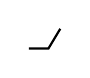
\begin{tikzpicture}[baseline=(current bounding box.south)]
        \draw[thick] (0,0) -- (0.25,0) -- (0.4,0.25);
    \end{tikzpicture}}}\!\!}

% Color definitions
\definecolor{kernelcolor}{RGB}{200,0,0}      % Red for K (kernels)
\definecolor{sobolevcolor}{RGB}{0,0,200}     % Blue for P (Sobolev)
\definecolor{theoremcolor}{RGB}{240,248,255} % Light blue for theorem boxes
\definecolor{definitioncolor}{RGB}{255,248,240} % Light orange for definitions

% Enhanced math commands
\newcommand{\E}{\mathbb{E}}
\DeclareMathOperator{\Var}{Var}
\newcommand{\indic}{\mathbb{1}}
\newcommand{\dd}{\,d}

% Colored operators
\newcommand{\Kop}{\textcolor{kernelcolor}{\mathbf{K}}}
\newcommand{\Pop}{\textcolor{sobolevcolor}{\mathbf{P}}}
\newcommand{\Kinf}{\textcolor{kernelcolor}{K^{\infty}}}
\newcommand{\Ps}{\textcolor{sobolevcolor}{P_s}}
\newcommand{\Ts}{\mathcal{T}_s}

% Beautiful theorem environments
\theoremstyle{plain}
\newtheorem{theorem}{Theorem}[section]
\newtheorem{lemma}[theorem]{Lemma}
\newtheorem{corollary}[theorem]{Corollary}
\newtheorem{proposition}[theorem]{Proposition}

\theoremstyle{definition}
\newtheorem{definition}[theorem]{Definition}
\newtheorem{example}[theorem]{Example}

\theoremstyle{remark}
\newtheorem*{remark}{Remark}

% Colored theorem boxes using tcolorbox
\tcolorboxenvironment{theorem}{
  colback=theoremcolor,
  colframe=blue!50!black,
  fonttitle=\bfseries,
  before skip=10pt,
  after skip=10pt,
  enhanced,
  drop shadow
}

\tcolorboxenvironment{definition}{
  colback=definitioncolor,
  colframe=orange!50!black,
  fonttitle=\bfseries,
  before skip=10pt,
  after skip=10pt,
  enhanced,
  drop shadow
}

\tcolorboxenvironment{lemma}{
  colback=green!5,
  colframe=green!50!black,
  fonttitle=\bfseries,
  before skip=8pt,
  after skip=8pt
}

\tcolorboxenvironment{corollary}{
  colback=purple!5,
  colframe=purple!50!black,
  fonttitle=\bfseries,
  before skip=8pt,
  after skip=8pt
}

\author{Janis AIAD}
\date{\today}
\title{Analysis of Deep Neural Network Learning Dynamics Through the NTK Lens}
\subtitle{Deeper or Wider ? A 1st answer under the NTK perspective}
% to change logo, add the image in PDF format
% or image by dragging it to the right and replace typographix
% with the image name, if you don't want a logo, 
% delete the line. 

\begin{figure*}[b]
    
\includegraphics[width=0.4\linewidth]{figures/umdlogo.jpg}
    \label{fig:enter-label}
\end{figure}


\fontsize{40pt}{48pt}

\begin{document}
	\maketitle 
	
	\tableofcontents
\newpage

\addcontentsline{toc}{section}{Abstract}
\section*{Abstract}
This report presents the results of a research internship focused on studying the learning dynamics of deep neural networks. We explore the underlying mechanisms through the Neural Tangent Kernel (NTK) formalism \cite{jacot2018neural}, with particular attention to finite-width corrections \cite{seleznova2022ntk_beyond}. Our work revolves around the decomposition of the NTK via Sobolev training, the analysis of its reproducing kernel Hilbert space (RKHS), and the study of extreme eigenvalues. We present theoretical bounds for the smallest eigenvalue of the NTK using random matrix theory (RMT) techniques. These results are then applied to analyze different architectures, including feed-forward neural networks (FCNN), matrix memory neural networks (MMNN), and transformers. We also discuss the implications of our findings for scientific machine learning (SciML) applications and propose directions for future research.

\newpage
\addcontentsline{toc}{section}{Executive summary}


\newpage
\addcontentsline{toc}{section}{Introduction}
\section*{Introduction}
The study of learning dynamics in deep neural networks constitutes a fundamental research area. Our approach focuses on the desingularization of Sobolev training by decomposing the problem into two distinct contributions: an independent neural tangent kernel (NTK) and a Sobolev contribution. This decomposition relies on the commutation between integral operators and the fractional Laplace operator.

\textbf{Key Discovery}: We establish that this commutation property holds \textit{exactly} only when using \textcolor{red}{\textbf{Chebyshev points}} (or equivalent optimal interpolation nodes) for sampling. For general sampling points, commutation breaks, necessitating explicit derivative information for effective learning. This fundamental distinction explains the empirical success of Physics-Informed Neural Networks (PINNs) and derivative-augmented methods over standard regression in most practical settings.

Our analysis continues with the study of NTK preconditioning through a freeze weights method, illustrated by neural networks factorizing low-rank weight matrices. This approach is supported by a rigorous approximation theorem. For classical feed-forward networks (FCNN), we develop a finite-width correction that proves particularly fruitful. Finally, we explore Transformers as an alternative solution, offering a new learning paradigm.

Across these different architectures, we study feature learning regimes and their scaling with network width. Our results rely on statistical physics tools to characterize model convergence and asymptotic behavior. This analysis enables a better understanding of finite-width corrections \cite{seleznova2022ntk_beyond} and their implications for the practical optimization of deep neural networks.


\newpage
\addcontentsline{toc}{section}{Notations}
\section*{Notations}

\begin{tcolorbox}[colback=blue!5,colframe=blue!50!black,title={\large \textbf{Mathematical Notation Reference}},enhanced,drop shadow]

\subsection*{Basic Mathematical Symbols}
\begin{longtable}{p{0.2\textwidth}p{0.15\textwidth}p{0.2\textwidth}p{0.15\textwidth}}
\toprule
\textbf{Symbol} & \textbf{Definition} & \textbf{Symbol} & \textbf{Definition} \\
\midrule
$\mathbb{R}$ & Set of real numbers & $\mathbb{N}$ & Set of natural numbers \\
$\mathbb{C}$ & Set of complex numbers & $\mathbb{S}^{d-1}$ & Unit sphere of dimension $d-1$ \\
$\E[\cdot]$ & Mathematical expectation & $\Var(\cdot)$ & Variance of a random variable \\
$\Cov(\cdot,\cdot)$ & Covariance between two variables & $\Corr(\cdot,\cdot)$ & Correlation between two variables \\
$\indic\{\cdot\}$ & Indicator function & $\dd x$ & Differential element \\
$\|\cdot\|$ & Euclidean norm & $\langle \cdot,\cdot \rangle$ & Inner product \\
$\mathcal{O}(\cdot)$ & Landau notation (big O) & $\tilde{\Omega}(\cdot)$ & Landau notation (big Omega tilde) \\
\bottomrule
\end{longtable}

\subsection*{Neural Network and Activation Functions}
\begin{longtable}{p{0.2\textwidth}p{0.15\textwidth}p{0.2\textwidth}p{0.15\textwidth}}
\toprule
\textbf{Symbol} & \textbf{Definition} & \textbf{Symbol} & \textbf{Definition} \\
\midrule
$\ReLU$ & ReLU activation function & $f(\mathbf{x}; \boldsymbol{\theta})$ & Neural network function \\
$\sigma(\cdot)$ & General activation function & $\sigma^2$ & Activation variance parameter \\
$L$ & Number of layers & $n_k$ & Width of layer $k$ \\
\bottomrule
\end{longtable}

\subsection*{Neural Tangent Kernel (NTK)}
\begin{longtable}{p{0.2\textwidth}p{0.15\textwidth}p{0.2\textwidth}p{0.15\textwidth}}
\toprule
\textbf{Symbol} & \textbf{Definition} & \textbf{Symbol} & \textbf{Definition} \\
\midrule
$\textcolor{kernelcolor}{\mathbf{K}}$ & Discrete NTK matrix & $\textcolor{kernelcolor}{K^{\infty}}$ & Infinite-width NTK operator \\
$K^{L}(\mathbf{x}_i, \mathbf{x}_j)$ & NTK for $L$-layer network & $\mu_\ell^{(K)}$ & NTK eigenvalues at degree $\ell$ \\
$\varrho(\rho)$ & Correlation propagation function & $\rho_1(\mathbf{x},\mathbf{x}')$ & Initial correlation \\
\bottomrule
\end{longtable}

\end{tcolorbox}

\begin{tcolorbox}[colback=blue!5,colframe=blue!50!black,title={\large \textbf{Mathematical Notation Reference}},enhanced,drop shadow]

\newpage
\subsection*{Sobolev Spaces and Training}
\begin{longtable}{p{0.2\textwidth}p{0.15\textwidth}p{0.2\textwidth}p{0.15\textwidth}}
\toprule
\textbf{Symbol} & \textbf{Definition} & \textbf{Symbol} & \textbf{Definition} \\
\midrule
$H^s(\Omega)$ & Sobolev space of order $s$ & $\textcolor{sobolevcolor}{\mathbf{P}}_s$ & Discrete Sobolev operator matrix \\
$P_s$ & Continuous Sobolev operator & $\mathcal{L}_{\text{Sobolev}}(f)$ & Sobolev training loss function \\
$D^k$ & $k$-th derivative operator & $\|f\|_{H^s}$ & Sobolev norm of order $s$ \\
$(I + (-\Delta)^{1/2})^s$ & Fractional Laplacian operator & $\Delta_{\mathbb{S}^{d-1}}$ & Laplace-Beltrami operator \\
\bottomrule
\end{longtable}

\subsection*{Spherical Harmonics and Fourier Analysis}
\begin{longtable}{p{0.2\textwidth}p{0.15\textwidth}p{0.2\textwidth}p{0.15\textwidth}}
\toprule
\textbf{Symbol} & \textbf{Definition} & \textbf{Symbol} & \textbf{Definition} \\
\midrule
$Y_{\ell,p}$ & Spherical harmonics & $N(d,\ell)$ & Multiplicity of harmonics \\
$\hat{f}(\xi)$ & Fourier transform of $f$ & $\xi$ & Frequency variable \\
$\sigma(x)$ & Surface measure on sphere & $\ell$ & Degree index \\
$p$ & Order index & $\nabla$ & Gradient operator \\
\bottomrule
\end{longtable}

\subsection*{Eigenvalues and Spectral Analysis}
\begin{longtable}{p{0.2\textwidth}p{0.15\textwidth}p{0.2\textwidth}p{0.15\textwidth}}
\toprule
\textbf{Symbol} & \textbf{Definition} & \textbf{Symbol} & \textbf{Definition} \\
\midrule
$\lambda_\ell$ & Eigenvalues at degree $\ell$ & $\lambda_{\min}(A)$ & Minimum eigenvalue \\
$\lambda_{\max}(A)$ & Maximum eigenvalue & $\mu_\ell^{(P_s)}$ & Sobolev eigenvalues \\
$C(d,L)$ & Constants depending on $d,L$ & $\Gamma(\cdot)$ & Gamma function \\
$P_\ell^{(\alpha)}(t)$ & Gegenbauer polynomials & $\tilde{K}_L^{\infty}(t)$ & Normalized NTK function \\
\bottomrule
\end{longtable}

\subsection*{Matrix Operations and Training}
\begin{longtable}{p{0.2\textwidth}p{0.15\textwidth}p{0.2\textwidth}p{0.15\textwidth}}
\toprule
\textbf{Symbol} & \textbf{Definition} & \textbf{Symbol} & \textbf{Definition} \\
\midrule
$A^T$ & Matrix transpose & $\|A\|_{op}$ & Operator norm \\
$\|A\|_F$ & Frobenius norm & $A \circ B$ & Hadamard product \\
$\mathcal{T}_s$ & Composite learning operator & $a_{\ell,p}$ & Sampling vectors \\
$\eta$ & Learning rate & $f_t(x)$ & Network at time $t$ \\
$y_i$ & Target output & $n$ & Number of samples \\
$d$ & Input dimension & $s$ & Sobolev order \\
\bottomrule
\end{longtable}

\end{tcolorbox}

\newpage



\subsection{Réseaux à Mémoire Matricielle (MMNN) et Transformeurs}
(Description des techniques de préconditionnement du NTK pour ces architectures. Discussion sur les régimes "feature" et "kernel", et sur les défis liés à l'optimisation. Présentation d'une conjecture sur la stabilité autour des minima globaux.)


\section{Model Definition and Asymptotic Regime}
This work derives the Neural Tangent Kernel (NTK) of a Multi-layer Mean-field Matrix-Normal Network (MMNN). The kernel is computed with respect to a specific set of trainable parameters, under the standard "NTK parameterization" which ensures a well-defined infinite-width limit.

\subsection{Multi-Layer MMNN Architecture}
We consider an MMNN of depth $L$. Let the input be $\bm{h}^{(0)}(\bm{x}) = \bm{x} \in \mathbb{R}^{d_0}$. For each layer $\ell = 1, \dots, L$, the output $\bm{h}^{(\ell)}$ is defined recursively:
\begin{equation}
    \bm{h}^{(\ell)}(\bm{x}) = \bm{c}^{(\ell)} + \frac{\sigma_A}{\sqrt{n_\ell}} \sum_{j=1}^{n_\ell} \bm{A}_j^{(\ell)} \sigma\left(\bm{w}_j^{(\ell)\top} \bm{h}^{(\ell-1)}(\bm{x}) + \beta b_j^{(\ell)}\right)
\end{equation}
where $n_\ell$ is the width of layer $\ell$ and $\bm{h}^{(\ell)} \in \mathbb{R}^{d_\ell}$.

The parameters for each layer are divided into two groups:
\begin{itemize}
    \item \textbf{Trainable Parameters:} The output weights $\{\bm{A}_j^{(\ell)}\}_{j=1}^{n_\ell}$ and biases $\bm{c}^{(\ell)}$ are optimized during training. The NTK is computed with respect to these parameters. They are initialized as follows:
    \begin{itemize}
        \item The weights $\bm{A}_j^{(\ell)}$ are drawn from a standard normal distribution, $\bm{A}_j^{(\ell)} \sim \mathcal{N}(0, 1)$. The term $\frac{\sigma_A}{\sqrt{n_\ell}}$ is the \textbf{NTK parameterization}, which ensures that the kernel converges as $n_\ell \to \infty$. The hyperparameter $\sigma_A$ controls the variance of the layer's output.
        \item The bias $\bm{c}^{(\ell)}$ is initialized at zero. For the kernel computation, its variance is taken as $\sigma_c^2 = 1$ for all layers.
    \end{itemize}
    \item \textbf{Random Parameters:} The input weights $\bm{w}_j^{(\ell)}$ and biases $b_j^{(\ell)}$ are randomly initialized and fixed throughout training. They are drawn from standard normal distributions: $\bm{w}_j^{(\ell)} \sim \mathcal{N}(0, \mathbf{I})$ and $b_j^{(\ell)} \sim \mathcal{N}(0, 1)$. The parameter $\beta$ controls the variance of the random bias term inside the activation. The choice of an isotropic distribution for the random weights is deliberate: the network is not designed with a bias for any specific input directions at any given layer. Instead, it learns to represent preferred directions by transforming the input space through the trainable parameters of the preceding layers. The output of layer $\ell-1$, $\bm{h}^{(\ell-1)}$, is already a structured, non-isotropic representation of the original data, and the isotropic random projections of layer $\ell$ act upon this learned representation.
\end{itemize}

\subsection{Parameterization and Training Regime}
The choice of scaling for the trainable parameters, known as the parameterization, critically determines the network's behavior in the infinite-width limit.
\begin{itemize}
    \item \textbf{NTK Parameterization (this work):} We use the $\frac{1}{\sqrt{n_\ell}}$ scaling. With this choice, the output function $h^{(\ell)}(x)$ has a variance of order $\mathcal{O}(\sigma_A^2)$, meaning its magnitude is stable as the width grows. However, the gradient of the function with respect to the non-scaled weights $\bm{A}_j^{(\ell)}$ is small, of order $\mathcal{O}(\frac{1}{\sqrt{n_\ell}})$. This leads to a "lazy training" regime where network parameters change very little during training. The network's dynamics can be accurately described by a linear model, whose kernel is the NTK.
    \item \textbf{Mean-Field (or \(\mu\)) Parameterization:} An alternative is to use a $\frac{1}{n_\ell}$ scaling. This would result in function outputs of order $\mathcal{O}(\frac{1}{\sqrt{n_\ell}})$ but gradients of order $\mathcal{O}(\frac{1}{n_\ell})$, which allows for more significant parameter movement and "feature learning," leading to a different, non-linear training dynamic.
\end{itemize}
Our use of the NTK parameterization is standard for deriving the NTK and analyzing the network at initialization.

\subsection{Asymptotic Regime}
The entire NTK and NNGP formalism relies on the infinite-width limit. Following the framework established by Jacot et al., we analyze the network in a specific asymptotic regime:
\begin{itemize}
    \item The dimensions of the hidden layers, or widths, $n_1, n_2, \dots, n_L$ are taken to infinity.
    \item The input and output dimensions of each layer ($d_0, d_1, \dots, d_L$) are kept fixed and finite.
    \item Critically, the limits are taken sequentially: first we let $n_1 \to \infty$, then $n_2 \to \infty$, and so on up to $n_L \to \infty$.
    \item In this limit, the output of each layer $h^{(\ell)}$ converges in distribution to a Gaussian Process (GP). Consequently, the NNGP and NTK kernels for layers $\ell > 1$, which are functions of the previous layer's output, remain random quantities (random fields). The recursive formulas describe the relationship between these random kernels.
\end{itemize}
This sequential limit is the key theoretical tool. When analyzing layer $\ell$ in the limit $n_\ell \to \infty$, the output of the previous layer, $\bm{h}^{(\ell-1)}$, is a sum of an infinite number of i.i.d. random variables (by construction of layer $\ell-1$). By the Central Limit Theorem, $\bm{h}^{(\ell-1)}$ converges in distribution to a Gaussian Process. This allows us to replace the complex, random function $\bm{h}^{(\ell-1)}$ with a GP whose covariance structure is precisely the NNGP kernel $\Sigma^{(\ell-1)}$. This is the foundation of the recursive calculation.

\section{Signal Propagation and the Edge of Chaos (EOC)}
Before analyzing the kernel, we study the propagation of the signal's magnitude through the network at initialization. We are interested in the evolution of the average variance per dimension of the layer outputs, defined as $q^{(\ell)} = \mathbb{E}[\|\bm{h}^{(\ell)}\|^2]/d_\ell$.

For a ReLU activation and assuming centered parameters, the variance evolves according to the following recurrence relation (see Appendix for proof):
\begin{equation}
    q^{(\ell)} = \sigma_c^2 + \frac{\sigma_A^2}{2} \left( q^{(\ell-1)}\text{Tr}(\Sigma_w) + \beta^2 \right)
\end{equation}
This is an affine map $q^{(\ell)} = M \cdot q^{(\ell-1)} + C$. For the signal to propagate stably without vanishing ($M<1$) or exploding ($M>1$), the dynamics must be at the "Edge of Chaos", where the multiplicative factor is exactly 1.

% \begin{block}
{Edge of Chaos Condition}

The condition for stable signal propagation is:
\begin{equation}
    \frac{\sigma_A^2}{2} \text{Tr}(\Sigma_w) = 1 \quad \implies \quad \sigma_A \sqrt{\text{Tr}(\Sigma_w)} = \sqrt{2}
\end{equation}
This establishes a critical relationship between the variance of the trainable weights ($\sigma_A^2$) and the trace of the random weight covariance matrix ($\Sigma_w$).
% \end{block}

\section{The NTK as a Guide to the Optimization Landscape}
A central motivation for studying the NTK is its direct connection to the optimization process. The NTK is the kernel of a linearized model of the neural network, and its properties dictate the local training dynamics under gradient descent.

\begin{itemize}
    \item \textbf{The NTK Governs Dynamics:} In the infinite-width limit, the gradient descent dynamics of a neural network are equivalent to kernel regression with the NTK. The spectrum of the NTK, particularly its condition number, determines the convergence rates.
    \item \textbf{A Proxy for the Hessian:} The NTK can be seen as a proxy for the Gauss-Newton approximation of the Hessian matrix. Crucially, the NTK is often much easier to compute and analyze than the full Hessian.
    \item \textbf{Choosing an Optimizer:} By analyzing the NTK's spectrum, we can make informed decisions about optimization strategy. An ill-conditioned NTK suggests that first-order methods (like gradient descent) are appropriate, while a well-conditioned NTK suggests that second-order methods (which use Hessian information) can converge much more rapidly.
    \item \textbf{From a Moving Kernel to Probabilistic Bounds:} Even though the MMNN's NTK is a random, evolving quantity (a "moving" kernel), our goal remains the same. By finding probabilistic laws that describe the distribution and evolution of the NTK's spectrum—either through mathematical analysis or numerical simulation—we can aim to derive optimization bounds. This allows us to understand, in a principled way, how the architectural choices in an MMNN affect its trainability.
\end{itemize}

\section{NTK for a Single-Layer MMFN}
\label{sec:single_layer_mmfn}
We begin by deriving the Neural Tangent Kernel for a single-layer Mean-field Matrix-Normal Network (MMFN). This result forms the base case for the multi-layer recursion. For simplicity, we consider a single scalar output, such that the network is defined as:
\begin{equation}
    h(\bm{x}) = \frac{1}{\sqrt{n}} \sum_{j=1}^n A_j \sigma(\bm{w}_j^\top \bm{x} + b_j) + c
\end{equation}
The trainable parameters are $\theta = \{A_j\}_{j=1}^n \cup \{c\}$. The parameters $\{\bm{w}_j, b_j\}$ are fixed and randomly drawn, with $\bm{w}_j \sim \mathcal{N}(0, \Sigma_w)$ and $b_j \sim \mathcal{N}(\mu_b, \sigma_b^2)$. While Gaussian distributions are used here for analytic tractability, the formalism can be extended to other distributions.

\subsection{From Gradient Products to an Expectation}
In the infinite-width limit ($n \to \infty$), the NTK converges to an expectation over the distribution of the random parameters $(\bm{w}, b)$. The full NTK is the sum of the kernel part from the weights $\{A_j\}$ and the part from the bias $\{c\}$.
\begin{equation}
\label{eq:ntk_expectation}
    \Theta^{(1)}(\bm{x}, \bm{x}') = \underbrace{\mathbb{E}_{\bm{w},b} \left[ \sigma(\bm{w}^\top \bm{x} + b)\sigma(\bm{w}^\top \bm{x}' + b) \right]}_{\text{NNGP Kernel } \Sigma^{(1)}(\bm{x}, \bm{x}')} + \underbrace{1}_{\text{from bias } c}
\end{equation}
The expectation term is exactly the Neural Network Gaussian Process (NNGP) kernel for this layer, which we denote $\Sigma^{(1)}$.

\subsection{Integral Formulation and Parameter Mapping}
The NNGP kernel $\Sigma^{(1)}$ is an integral over the distributions of $\bm{w}$ and $b$:
\begin{equation}
    \Sigma^{(1)}(\bm{x}, \bm{x}') = \int_{\mathbb{R}^d} \int_{\mathbb{R}} \sigma(\bm{w}^\top \bm{x} + b)\sigma(\bm{w}^\top \bm{x}' + b) p(\bm{w})p(b) \,db \,d\bm{w}
\end{equation}
where $p(\bm{w})$ and $p(b)$ are the probability density functions. A change of variables is performed from the parameter space $(\bm{w}, b)$ to the pre-activation space $(g_1, g_2)$, where $g_1 = \bm{w}^\top \bm{x} + b$ and $g_2 = \bm{w}^\top \bm{x}' + b$. This transforms the high-dimensional integral into an expectation over a 2D bivariate Gaussian distribution. The parameters of this distribution are:
\begin{itemize}
    \item \textbf{Means:} $\mu_1 = \mathbb{E}[g_1] = \mathbb{E}[\bm{w}^\top\bm{x} + b] = \mu_b$. By symmetry, $\mu_2 = \mu_b$.
    \item \textbf{Variances:} $\sigma_1^2 = \text{Var}(g_1) = \text{Var}(\bm{w}^\top\bm{x}) + \text{Var}(b) = \bm{x}^\top \Sigma_w \bm{x} + \sigma_b^2$. Similarly, $\sigma_2^2 = {\bm{x}'}^\top \Sigma_w \bm{x}' + \sigma_b^2$.
    \item \textbf{Covariance:} $\text{Cov}(g_1, g_2) = \mathbb{E}[(\bm{w}^\top\bm{x})(\bm{w}^\top\bm{x}')] + \text{Var}(b) = \bm{x}^\top \Sigma_w \bm{x}' + \sigma_b^2$.
\end{itemize}

\subsection{Final Analytical Expression}
\begin{theorem}[NNGP Kernel for a Single-Layer ReLU MMFN]
Let the pre-activations $(g_1, g_2)$ be jointly Gaussian with parameters $(\mu_1, \sigma_1^2)$ and $(\mu_2, \sigma_2^2)$ and correlation $\rho$. The NNGP kernel $\Sigma^{(1)} = \mathbb{E}[\text{ReLU}(g_1)\text{ReLU}(g_2)]$ is given by the decomposition:
\begin{equation}
\label{eq:final_ntk_decomp}
\boxed{
\Sigma^{(1)} = \sigma_1\sigma_2 \cdot I_{12} + \mu_1\sigma_2 \cdot I_{01} + \mu_2\sigma_1 \cdot I_{10} + \mu_1\mu_2 \cdot I_{00}
}
\end{equation}
where the terms $I_{ij}$ are moments of standardized bivariate normal variables $(Z_1, Z_2)$ with thresholds $a_1 = -\mu_1/\sigma_1$ and $a_2 = -\mu_2/\sigma_2$. These moments and their analytical solutions are well-known in the literature.
\end{theorem}

\subsubsection{Detailed Kernel Computation via Nested Expectation}
The general formula can be analyzed more deeply under specific parameterizations. A common and insightful case is when the random features are normalized. Assume the network's pre-activation is $g(\bm{x}) = Q(\bm{x}) + \beta b$, where $Q(\bm{x})$ is a zero-mean Gaussian process with unit variance ($\mathbb{E}[Q(\bm{x})^2]=1$) and $b \sim \mathcal{N}(0,1)$ is an independent random bias. For two inputs $\bm{x}, \bm{x}'$, the random variables $(Q(\bm{x}), Q(\bm{x}'))$ follow a centered bivariate normal distribution with correlation $\rho = \mathbb{E}[Q(\bm{x})Q(\bm{x}')]$.

The NNGP kernel $\Sigma^{(1)}$ is then a nested expectation:
\begin{equation}
    \Sigma^{(1)}(\rho, \beta) = \mathbb{E}_{b} \left[ \mathbb{E}_{Q_1, Q_2} \left[ \sigma(Q_1 + \beta b) \sigma(Q_2 + \beta b) \right] \right]
\end{equation}
where $(Q_1, Q_2) \sim \mathcal{N}(0, \begin{psmallmatrix} 1 & \rho \\ \rho & 1 \end{psmallmatrix})$.

For a fixed $b$, the inner expectation is over two ReLU functions whose arguments are non-centered Gaussians with mean $\mu = \beta b$ and variance $1$. This inner expectation, let's call it $\mathcal{I}(\mu, \rho)$, can be decomposed using moments of a standardized bivariate normal distribution:
\begin{equation}
    \mathcal{I}(\mu, \rho) = I_2(\mu, \rho) + 2\mu I_1(\mu, \rho) + \mu^2 I_0(\mu, \rho)
\end{equation}
where $a = -\mu = -\beta b$ is the truncation threshold. The moment functions are:
\begin{itemize}
    \item \textbf{Zeroth Moment (Probability):} $I_0(\mu, \rho) = \mathbb{P}(Q_1 > a, Q_2 > a) = L(a, a; \rho)$, where $L$ is the bivariate normal survival function.
    \item \textbf{First Moment:} $I_1(\mu, \rho) = \mathbb{E}[Q_1 \cdot \mathbf{1}_{Q_1>a, Q_2>a}] = (1+\rho)\phi(a)\Phi\left(a\sqrt{\frac{1-\rho}{1+\rho}}\right)$.
    \item \textbf{Second Moment:} $I_2(\mu, \rho) = \mathbb{E}[Q_1 Q_2 \cdot \mathbf{1}_{Q_1>a, Q_2>a}] = \rho L(a, a; \rho) + (1-\rho^2)\phi(a, a; \rho)$, where $\phi(\cdot,\cdot;\rho)$ is the bivariate normal PDF.
\end{itemize}
The total kernel is then found by taking the expectation over $b$, which results in a one-dimensional integral:
\begin{equation}
    \Sigma^{(1)}(\rho, \beta) = \int_{-\infty}^{\infty} \mathcal{I}(\beta b, \rho) \, \phi(b) \, db
\end{equation}
where $\phi(b)$ is the standard normal PDF. This formulation is what is implemented for numerical computation.

\section{Recursion for Multi-Layer MMNNs}
We now extend the single-layer result to deep networks. The recursion involves two distinct but intertwined kernels: the NNGP kernel $\Sigma^{(\ell)}$ and the NTK kernel $\Theta^{(\ell)}$.

\subsection{The Critical Role of the $({w}^\top{w}$ Term in the Derivative Kernel}
The recursive formula for the NTK, $\Theta^{(\ell)} = \Theta^{(\ell-1)} \cdot \sigma_A^2 \dot{\Sigma}^{(\ell)} + \dots$, shows that the derivative kernel $\dot{\Sigma}^{(\ell)}$ governs the propagation of gradient information through the layers. Its definition contains a crucial term:
\[ \dot{\Sigma}^{(\ell)}(x, x') = \mathbb{E}_{\bm{w}, b} \left[ \dot{\sigma}(\dots) \dot{\sigma}(\dots) \bm{w}^\top\bm{w} \right] \]
The presence of the inner product $\bm{w}^\top\bm{w}$ (the squared Euclidean norm of the random weight vector) is of paramount importance. For isotropic Gaussian weights, its expectation is $\mathbb{E}[\bm{w}^\top\bm{w}] = d_{\ell-1}$, the dimension of the previous layer's output. This introduces a factor proportional to the network's width at each layer into the recursive term of the NTK.

\textbf{This can lead to a much faster, potentially explosive, growth of the NTK's magnitude with depth compared to the NNGP kernel.} A precise mathematical investigation of how this term interacts with the rest of the expectation is therefore essential to correctly characterize the scaling laws of the NTK in deep MMNNs, and will be a central part of our future work.

\subsection{Remark on Model Structure and the Role of \(\beta\)}
A key feature of this model is the structure of the pre-activation at each layer: $g = \bm{w}^\top \bm{h}_{in} + \beta b$. This structure, where $\bm{w}$ and $b$ are random parameters, is central to the model's behavior. It introduces two sources of randomness that are propagated through the network:
\begin{enumerate}
    \item \textbf{Function-space Randomness:} In the infinite-width limit, the output of each layer is a random function drawn from a Gaussian Process, whose covariance is the NNGP kernel $\Sigma^{(\ell)}$.
    \item \textbf{Parameter Randomness:} The explicit random parameter $b$, scaled by $\beta$, inside the non-linearity adds another layer of randomness. It ensures that the pre-activation remains a random variable even if the layer's input becomes deterministic. 
\end{enumerate}
This implies that the function inside the expectation of the $\mathcal{L}$ operator is not just the activation $\sigma(\cdot)$, but represents the entire operation whose statistics are captured by the recursive kernel definitions below.

\subsection{NNGP Kernel \(\Sigma^{(\ell)}\) Recursion}
The NNGP kernel describes the covariance of the network's output function at initialization. For any finite width, this output is a random function. In the infinite-width limit, it converges to a Gaussian Process. The base kernel $\Sigma^{(\ell)}$ is defined recursively.
\begin{itemize}
    \item \textbf{Base Case (\(\ell=1\)):} The NNGP kernel for the first layer, $\Sigma^{(1)}$, corresponds to the expectation part of the single-layer kernel theorem.
    \begin{equation}
        \Sigma^{(1)}(x, x') = \mathbb{E}_{\bm{w},b}\left[\sigma(\bm{w}^\top x + b)\sigma(\bm{w}^\top x' + b)\right]
    \end{equation}
    
    \item \textbf{Recursive Step (\(\ell > 1\)):} For subsequent layers, the base kernel $\Sigma^{(\ell)}$ is defined by taking the expectation only over the random parameters of the current layer ($\bm{w}, b$), for a given realization of the previous layer's output GP $\bm{h}^{(\ell-1)}$.
    \begin{equation}
        \Sigma^{(\ell)}(x, x') = \mathbb{E}_{\bm{w}, b} \left[ \sigma\left(\bm{w}^\top \bm{h}^{(\ell-1)}(x) + \beta b\right) \sigma\left(\bm{w}^\top \bm{h}^{(\ell-1)}(x') + \beta b\right) \right]
    \end{equation}
    Since $\bm{h}^{(\ell-1)}$ is itself a random GP, the resulting kernel $\Sigma^{(\ell)}$ is a random quantity for $\ell > 1$.
    To be precise, the expectation over $\bm{h}^{(\ell-1)}$ is taken over a joint Gaussian distribution. Since $\bm{h}^{(\ell-1)}$ is a $d_{\ell-1}$-dimensional Gaussian Process, for any pair of inputs $x, x'$, the concatenated vector $(\bm{h}^{(\ell-1)}(x), \bm{h}^{(\ell-1)}(x'))$ follows a $2d_{\ell-1}$-dimensional Gaussian distribution. Assuming the outputs of layer $\ell-1$ are i.i.d. GPs, the covariance matrix of this vector has a block structure:
\end{itemize}

\subsection{NTK Kernel \(\Theta^{(\ell)}\) Recursion}
The NTK is the Gram matrix of function gradients. For any finite width, it is a random matrix. The following recursion describes the relationship between these random kernels in the infinite-width limit.
\begin{itemize}
    \item \textbf{Initialization (\(\ell=0\)):} The recursion starts with $\Theta^{(0)} = 0$.
    
    \item \textbf{Recursive Step (\(\ell \ge 1\)):} The NTK for layer $\ell$ combines the NTK from previous layers with the contributions from the trainable parameters of the current layer, $A^{(\ell)}$ and $c^{(\ell)}$.
    \begin{equation}
        \boxed{
        \Theta^{(\ell)}(x, x') = \Theta^{(\ell-1)}(x, x') \cdot \left(\sigma_A^2\dot{\Sigma}^{(\ell)}(x, x')\right) + \Sigma^{(\ell)}(x, x') + 1
        }
    \end{equation}
    Here, $\sigma_c^2=1$ is the contribution from the trainable bias. $\Sigma^{(\ell)}$ is the base NNGP kernel defined above. $\dot{\Sigma}^{(\ell)}$ is the base derivative kernel, defined similarly as an expectation over layer-$\ell$ parameters:
    \begin{equation}
        \dot{\Sigma}^{(\ell)}(x, x') = \mathbb{E}_{\bm{w}, b} \left[ \dot{\sigma}\left(\bm{w}^\top \bm{h}^{(\ell-1)}(x) + \beta b\right) \dot{\sigma}\left(\bm{w}^\top \bm{h}^{(\ell-1)}(x') + \beta b\right) \bm{w}^\top\bm{w} \right]
    \end{equation}
    with $\dot{\sigma}$ being the derivative of the activation function. Both $\Sigma^{(\ell)}$ and $\dot{\Sigma}^{(\ell)}$ are random kernels for $\ell > 1$.
\end{itemize}
This formulation now correctly incorporates the contribution of all trainable parameters at each layer.

\section{Summary of Formulas}
\vspace{1em}
\fbox{\begin{minipage}{0.95\textwidth}
\begin{itemize}
    \item \textbf{Layer Output:}
    \[ \bm{h}^{(\ell)}(\bm{x}) = \bm{c}^{(\ell)} + \frac{\sigma_A}{\sqrt{n_\ell}} \sum_{j=1}^{n_\ell} \bm{A}_j^{(\ell)} \sigma\left(\bm{w}_j^{(\ell)\top} \bm{h}^{(\ell-1)}(\bm{x}) + \beta b_j^{(\ell)}\right) \]

    \item \textbf{NNGP Kernel Recursion:}
    \begin{itemize}
        \item \textit{Base Kernel:} Expectation over current layer's random parameters, conditioned on the previous layer's output GP $\bm{h}^{(\ell-1)}$.
        \[ \Sigma^{(\ell)}(x, x') = \mathbb{E}_{\bm{w}, b} \left[ \sigma\left(\bm{w}^\top \bm{h}^{(\ell-1)}(x) + \beta b\right) \sigma\left(\bm{w}^\top \bm{h}^{(\ell-1)}(x') + \beta b\right) \right] \]
        \item \textit{Full Kernel:}
        \[ \mathcal{K}_{\text{NNGP}}^{(\ell)}(x, x') = \sigma_A^2 \Sigma^{(\ell)}(x, x') + \sigma_c^2 \]
    \end{itemize}

    \item \textbf{NTK Kernel Recursion:}
    \begin{itemize}
        \item \textit{Base Derivative Kernel:}
        \[ \resizebox{\textwidth}{!}{$\dot{\Sigma}^{(\ell)}(x, x') = \mathbb{E}_{\bm{w}, b} \left[ \dot{\sigma}\left(\bm{w}^\top \bm{h}^{(\ell-1)}(x) + \beta b\right) \dot{\sigma}\left(\bm{w}^\top \bm{h}^{(\ell-1)}(x') + \beta b\right) \bm{w}^\top\bm{w} \right]$} \]
        \item \textit{Full Kernel:}
        \[ \Theta^{(\ell)}(x, x') = \Theta^{(\ell-1)}(x, x') \cdot \sigma_A^2  \dot{\Sigma}^{(\ell)}(x, x') + \Sigma^{(\ell)}(x, x')+1 \]
    \end{itemize}
\end{itemize}
\end{minipage}}
\vspace{1em}


\section{Conclusion: A New Paradigm for NTK Analysis}
The analysis of MMNNs through the lens of NTK theory reveals a fascinating trade-off and a path toward a more general framework. Standard NTK theory for MLPs requires massive overparameterization (quadratic in width) to guarantee a static kernel and a "lazy training" regime. MMNNs offer a compelling alternative: it may be possible to enter an analyzable, NTK-like regime with a parameter count that is merely linear in the width.

The price for this parameter efficiency is that the kernel is no longer a deterministic, static object but a random field that evolves during training. However, this is not an insurmountable obstacle. The path forward is to embrace this randomness and analyze it using the tools of high-dimensional probability. By deriving concentration bounds (e.g., using Bernstein-type inequalities) on the spectrum and evolution of this random kernel, we can obtain robust, probabilistic guarantees on the optimization landscape. This provides a rigorous framework for understanding the benefits of the structural priors imposed by the MMNN architecture, moving beyond the idealized lazy training regime.

\section{Outlook: Application to PINNs and an Analogy to Wavelets}
A major potential application for this research lies in the field of Physics-Informed Neural Networks (PINNs). PINNs solve Partial Differential Equations (PDEs) by training a neural network to satisfy the governing equations. The core of this task is efficient function approximation. Since MMNNs are explicitly inspired by function decomposition theorems, their architecture is naturally suited for this purpose.

Furthermore, we can draw a powerful analogy between MMNNs and wavelet transforms, especially in the high-dimensional regime where the benefits become most apparent. A wavelet transform decomposes a function onto a fixed basis of localized functions. An MMNN performs a similar task, but learns the optimal combination of a rich, random basis of functions. Classical wavelet transforms suffer from the curse of dimensionality, making them intractable for high-dimensional problems.

The MMNN architecture overcomes this limitation through several mechanisms. In high dimensions, random vectors are nearly orthogonal, meaning the correlation $\rho$ between pre-activations of distinct inputs concentrates around zero. The Funk-Hecke theorem provides a powerful tool to analyze the kernel operator in this setting, showing that a kernel depending only on $\rho$ will have a highly structured spectrum. This concentration of $\rho$ implies that the NTK matrix itself becomes quasi-diagonal or takes on the simple $(a-b)\mathbf{I} + b\mathbf{J}$ structure, making its spectrum much easier to understand. The network effectively performs an automatic, adaptive directional domain decomposition. While the number of regions partitioned by the neurons can grow exponentially, the number of parameters only scales linearly with the width. This combination of expressive power and parameter efficiency makes the MMNN a powerful and tractable tool for applications like PINNs in high dimensions, where classical methods like wavelets fail.

A concrete step in this direction is to ensure the network has sufficient regularity. Many PDEs involve second-order derivatives (e.g., the Laplacian). To apply rigorous optimization and approximation theorems in this context, the network function must be twice-differentiable ($C^2$). A promising future direction is therefore to develop a "Deep Smooth ReLU Network" (DSRN) version of the MMNN, for instance by using smoother activation functions, which would guarantee the necessary regularity and unlock a wider range of theoretical tools for PINN analysis.

\section{Future Work}
The initial results are promising and open several avenues for both numerical and theoretical investigation.

\subsection{Numerical Investigations}
\begin{itemize}
    \item \textbf{Integration Accuracy:} Increase the network width/rank used for numerical integration to confirm that the observed phenomena are stable as we better approach the infinite-width limit.
\end{itemize}

\subsection{Mathematical Investigations}
A primary focus of future theoretical work will be to precisely characterize the spectrum of the MMNN's NTK operator using a trifecta of advanced analytical techniques. Before diving into these, we note an important methodological choice regarding the random bias.
\begin{itemize}
    \item \textbf{Role of the Bias Parameter $\beta$ and Simplified Regimes:} Our analysis has consistently included the random bias term $\beta b$, which makes the pre-activations non-centered and is a core feature of the MMNN model. However, for mathematical tractability, it is common in the NTK literature for MLPs to first analyze the system in a simplified, bias-free regime ($\beta=0$). This path offers two avenues:
        \begin{itemize}
            \item Analyze the kernel at $\beta=0$. While losing the specific non-centered interpretation, this could yield cleaner mathematical results as a first step.
            \item Perform a Taylor expansion (développement limité) of the kernel functions with respect to $\beta$ around $\beta=0$. This would allow us to systematically study the impact of the random bias perturbatively and bridge the gap between the simplified and the full model.
        \end{itemize}
\end{itemize}
The primary analytical approaches for the spectrum are:
\begin{itemize}
    \item \textbf{Spectrum via Puiseux Series Expansion:} Following the work of Bietti and Bach~\cite{bietti2021deepequalsshallowrelu}, we can analyze the Puiseux series expansion of the kernel function in the limits $\rho \to 1^-$ and $\rho \to -1^+$. The first non-integer exponent in this series expansion directly characterizes the asymptotic scaling of the NTK operator's eigenvalues.
    \item \textbf{Spectrum as a Zonal Operator:} A powerful approach is to analyze the NTK as a zonal kernel operator on the sphere. Following the methodology of Murray et al.~\cite{murray2023characterizingspectrumntkpower}, we can seek a power series expansion of the kernel in terms of the Gram matrix ($K = \bm{x}^\top\bm{x}'$). This would allow for a direct characterization of its eigenvalues in terms of Gegenbauer polynomials.
    \item \textbf{Spectrum vs. Depth Analysis:} Adapt the proof methodology from Terj\'{e}k and Gonz\'{a}lez-S\'{a}nchez~\cite{terjek2025mlpseocspectrumntk} to analyze how the NTK spectrum scales with depth $L$. This involves performing a power expansion of the kernel function with respect to the correlation $\rho$.
\end{itemize}
Further mathematical goals include:
\begin{itemize}
    \item \textbf{Connect to Function Decomposition:} Investigate using a uniform distribution for the random weights $\bm{w}$. This choice may align better with the function approximation theory that originally motivated the MMNN architecture. The intuition is that pairs of weights with opposite signs (e.g., $\bm{w}$ and $-\bm{w}$) could create basis functions that compensate for each other, effectively building localized basis functions over intervals defined by the pre-activations—a cornerstone of function decomposition.
    \item \textbf{Scaling Law Coefficient:} Derive the analytical form of the scaling law coefficient $C_{\text{scaling}}$ from Experiment 2 and determine its dependency on hyperparameters like $\sigma_A$ and $\beta$.
    \item \textbf{Rank-Magnitude Relationship:} Provide a rigorous theoretical explanation for the inverse relationship between layer rank and NTK magnitude, possibly leveraging Gaussian concentration of measure principles.
    \item \textbf{Constant Sine Kernel:} Investigate the analytical formulas for the Sine NTK to explain why it becomes nearly constant in our experimental setup, likely by analyzing the behavior of the correlation term $\rho$.
    \item \textbf{Theory of Evolving Kernels:} Develop a formal framework for analyzing the dynamics of the low-rank NTK, proving that it remains well-conditioned throughout training under certain assumptions.
    \item \textbf{Analysis of Trainable Activations (PSinTU):} A further avenue is to explore more expressive, trainable activation functions like Parametrized Sinusoidal Transform Unit (PSinTU). While this offers greater flexibility, the NTK analysis becomes significantly more complex as the basis functions themselves are no longer fixed. This will be tackled in a later phase of the research.
\end{itemize}





\subsection{Asymptotic Regime}
The entire NTK and NNGP formalism relies on the infinite-width limit. Following the framework established by Jacot et al., we analyze the network in a specific asymptotic regime:
\begin{itemize}
    \item The dimensions of the hidden layers, or widths, $n_1, n_2, \dots, n_L$ are taken to infinity.
    \item The input and output dimensions of each layer ($d_0, d_1, \dots, d_L$) are kept fixed and finite.
    \item Critically, the limits are taken sequentially: first we let $n_1 \to \infty$, then $n_2 \to \infty$, and so on up to $n_L \to \infty$.
    \item In this limit, the output of each layer $h^{(\ell)}$ converges in distribution to a Gaussian Process (GP). Consequently, the NNGP and NTK kernels for layers $\ell > 1$, which are functions of the previous layer's output, remain random quantities (random fields). The recursive formulas describe the relationship between these random kernels.
\end{itemize}
This sequential limit is the key theoretical tool. When analyzing layer $\ell$ in the limit $n_\ell \to \infty$, the output of the previous layer, $\bm{h}^{(\ell-1)}$, is a sum of an infinite number of i.i.d. random variables (by construction of layer $\ell-1$). By the Central Limit Theorem, $\bm{h}^{(\ell-1)}$ converges in distribution to a Gaussian Process. This allows us to replace the complex, random function $\bm{h}^{(\ell-1)}$ with a GP whose covariance structure is precisely the NNGP kernel $\Sigma^{(\ell-1)}$. This is the foundation of the recursive calculation.

\section{NTK for a Single-Layer MMFN}
\label{sec:single_layer_mmfn}
We begin by deriving the Neural Tangent Kernel for a single-layer Mean-field Matrix-Normal Network (MMFN). This result forms the base case for the multi-layer recursion. For simplicity, we consider a single scalar output, such that the network is defined as:
\begin{equation}
    h(\bm{x}) = \frac{1}{\sqrt{n}} \sum_{j=1}^n A_j \sigma(\bm{w}_j^\top \bm{x} + b_j) + c
\end{equation}
The trainable parameters are $\theta = \{A_j\}_{j=1}^n \cup \{c\}$. The parameters $\{\bm{w}_j, b_j\}$ are fixed and randomly drawn, with $\bm{w}_j \sim \mathcal{N}(0, \Sigma_w)$ and $b_j \sim \mathcal{N}(\mu_b, \sigma_b^2)$. While Gaussian distributions are used here for analytic tractability, the formalism can be extended to other distributions.

\subsection{From Gradient Products to an Expectation}
In the infinite-width limit ($n \to \infty$), the NTK converges to an expectation over the distribution of the random parameters $(\bm{w}, b)$. The full NTK is the sum of the kernel part from the weights $\{A_j\}$ and the part from the bias $\{c\}$.
\begin{equation}
\label{eq:ntk_expectation}
    \Theta^{(1)}(\bm{x}, \bm{x}') = \underbrace{\mathbb{E}_{\bm{w},b} \left[ \sigma(\bm{w}^\top \bm{x} + b)\sigma(\bm{w}^\top \bm{x}' + b) \right]}_{\text{NNGP Kernel } \Sigma^{(1)}(\bm{x}, \bm{x}')} + \underbrace{\sigma_c^2}_{\text{from bias } c}
\end{equation}
The expectation term is exactly the Neural Network Gaussian Process (NNGP) kernel for this layer, which we denote $\Sigma^{(1)}$.

\subsection{Integral Formulation and Parameter Mapping}
The NNGP kernel $\Sigma^{(1)}$ is an integral over the distributions of $\bm{w}$ and $b$:
\begin{equation}
    \Sigma^{(1)}(\bm{x}, \bm{x}') = \int_{\mathbb{R}^d} \int_{\mathbb{R}} \sigma(\bm{w}^\top \bm{x} + b)\sigma(\bm{w}^\top \bm{x}' + b) p(\bm{w})p(b) \,db \,d\bm{w}
\end{equation}
where $p(\bm{w})$ and $p(b)$ are the probability density functions. A change of variables is performed from the parameter space $(\bm{w}, b)$ to the pre-activation space $(g_1, g_2)$, where $g_1 = \bm{w}^\top \bm{x} + b$ and $g_2 = \bm{w}^\top \bm{x}' + b$. This transforms the high-dimensional integral into an expectation over a 2D bivariate Gaussian distribution. The parameters of this distribution are:
\begin{itemize}
    \item \textbf{Means:} $\mu_1 = \mathbb{E}[g_1] = \mathbb{E}[\bm{w}^\top\bm{x} + b] = \mu_b$. By symmetry, $\mu_2 = \mu_b$.
    \item \textbf{Variances:} $\sigma_1^2 = \text{Var}(g_1) = \text{Var}(\bm{w}^\top\bm{x}) + \text{Var}(b) = \bm{x}^\top \Sigma_w \bm{x} + \sigma_b^2$. Similarly, $\sigma_2^2 = {\bm{x}'}^\top \Sigma_w \bm{x}' + \sigma_b^2$.
    \item \textbf{Covariance:} $\text{Cov}(g_1, g_2) = \mathbb{E}[(\bm{w}^\top\bm{x})(\bm{w}^\top\bm{x}')] + \text{Var}(b) = \bm{x}^\top \Sigma_w \bm{x}' + \sigma_b^2$.
\end{itemize}

\subsection{Final Analytical Expression}
\begin{theorem}[NNGP Kernel for a Single-Layer ReLU MMFN]
Let the pre-activations $(g_1, g_2)$ be jointly Gaussian with parameters $(\mu_1, \sigma_1^2)$ and $(\mu_2, \sigma_2^2)$ and correlation $\rho$. The NNGP kernel $\Sigma^{(1)} = \mathbb{E}[\text{ReLU}(g_1)\text{ReLU}(g_2)]$ is given by the decomposition:
\begin{equation}
\label{eq:final_ntk_decomp}
\boxed{
\Sigma^{(1)} = \sigma_1\sigma_2 \cdot I_{12} + \mu_1\sigma_2 \cdot I_{01} + \mu_2\sigma_1 \cdot I_{10} + \mu_1\mu_2 \cdot I_{00}
}
\end{equation}
where the terms $I_{ij}$ are moments of standardized bivariate normal variables $(Z_1, Z_2)$ with thresholds $a_1 = -\mu_1/\sigma_1$ and $a_2 = -\mu_2/\sigma_2$. These moments and their analytical solutions are well-known in the literature.
\end{theorem}







\section{Recursion for Multi-Layer MMNNs}
We now extend the single-layer result to deep networks. The recursion involves two distinct but intertwined random fields: the NNGP kernel $\Sigma^{(\ell)}$ and the NTK kernel $\Theta^{(\ell)}$.
An important fact is that the NNGP kernel $\Sigma^{(\ell)}$ is a random field that is NOT a gaussian process but a deep gaussian process, while the NTK kernel $\Theta^{(\ell)}$ is also a random field that is not a gaussian process.

\subsection{Remark on Model Structure and the Role of \(\beta\)}
A key feature of this model is the structure of the pre-activation at each layer: $g = \bm{w}^\top \bm{h}_{in} + \beta b$. This structure, where $\bm{w}$ and $b$ are random parameters, is central to the model's behavior. It introduces two sources of randomness that are propagated through the network:
\begin{enumerate}
    \item \textbf{Function-space Randomness:} In the infinite-width limit, the output of each layer is a random function drawn from a Gaussian Process, whose covariance is the NNGP kernel $\Sigma^{(\ell)}$.
    \item \textbf{Parameter Randomness:} The explicit random parameter $b$, scaled by $\beta$, inside the non-linearity adds another layer of randomness. It ensures that the pre-activation remains a random variable even if the layer's input becomes deterministic. 
\end{enumerate}
This implies that the function inside the expectation of the $\mathcal{L}$ operator is not just the activation $\sigma(\cdot)$, but represents the entire operation whose statistics are captured by the recursive kernel definitions below.

\subsection{NNGP Kernel \(\Sigma^{(\ell)}\) Recursion}
The NNGP kernel describes the covariance of the network's output function at initialization. For any finite width, this output is a random function. In the infinite-width limit, it converges to a Gaussian Process. The base kernel $\Sigma^{(\ell)}$ is defined recursively.
\begin{itemize}
    \item \textbf{Base Case (\(\ell=1\)):} The NNGP kernel for the first layer, $\Sigma^{(1)}$, corresponds to the expectation part of the single-layer kernel theorem.
    \begin{equation}
        \Sigma^{(1)}(x, x') = \mathbb{E}_{\bm{w},b}\left[\sigma(\bm{w}^\top x + b)\sigma(\bm{w}^\top x' + b)\right]
    \end{equation}
    \item \textbf{Recursive Step (\(\ell > 1\)):} For subsequent layers, the base kernel $\Sigma^{(\ell)}$ is defined by taking the expectation only over the random parameters of the current layer ($\bm{w}, b$), for a given realization of the previous layer's output GP $\bm{h}^{(\ell-1)}$.
    \begin{equation}
        \Sigma^{(\ell)}(x, x') = \mathbb{E}_{\bm{w}, b} \left[ \sigma\left(\bm{w}^\top \bm{h}^{(\ell-1)}(x) + \beta b\right) \sigma\left(\bm{w}^\top \bm{h}^{(\ell-1)}(x') + \beta b\right) \right] 
        % }
    \end{equation}
    and for the full NNGP kernel, we have
    \begin{equation}
        \boxed{
        \mathcal{K}_{NNGP}^{(\ell)}=\sigma_A^2\Sigma^{(\ell-1)}+\sigma_c^2
        }
    \end{equation}
    Because $\bm{h}^{(\ell-1)}$ is a GP with kernel $\mathcal{K}_{NNGP}^{(\ell-1)}$, this expression defines a transformation that maps the kernel of layer $\ell-1$ to the kernel of layer $\ell$. For specific choices of distributions and activation functions (like Gaussians and ReLU), this expectation can be computed, often leading to a recursive formula expressed in terms of an operator acting on $\Sigma^{(\ell-1)}$.

    It's important to notice that this kernel becomes random and non-deterministic for $\ell >1$.

    \paragraph{Remark on the non-propagation of the Gaussian Process property.}
    It is crucial to understand how the Gaussian Process property is not maintained from layer to layer. 
    
    The composition of a non-linear function with a Gaussian Process, $g(f(x))$, is not, in general, a Gaussian Process. In our model, while $\bm{h}^{(\ell-1)}$ is a GP, the output of the non-linear activation, $\sigma(\bm{w}^\top \bm{h}^{(\ell-1)} + \beta b)$, is not.
   
    In general, if you want to compute the mean value of this deep gaussian process, you need to compute the expectation over the random field of the previous layer by conditioning on the random field of the previous layer.
    which means to change $\mathbb{E}_{\bm{w}, b} \left[ \dots \right]$ to $\mathbb{E}_{\bm{w}, b, \bm{h}^{(\ell-1)}} \left[ \dots \right]$.

    So the NNGP kernel that is defined is not the same as the NNGP that you can compute for MLPs, because the NNGP of MLPs is a gaussian process, while the NNGP of MMNNs is a deep gaussian process.
\end{itemize}

\subsection{NTK Kernel \(\Theta^{(\ell)}\) Recursion}
The NTK is the Gram matrix of function gradients with respect to the trainable parameters. For any finite width, it is a random matrix because it depends on the specific parameter initialization. The following recursion describes its deterministic limit, $\Theta^{(\ell)}$, as the layer widths tend sequentially to infinity.

We recall then that the NTK is a random field that is not a gaussian process. 
We compose gaussian processes in the definition of $\Sigma_{\ell}$ and  $\dot{\Sigma}^{(\ell)}$.


\begin{itemize}
    \item \textbf{Initialization (\(\ell=0\)):} The recursion starts with $\Theta^{(0)} = 0$.
    
    \item \textbf{Recursive Step (\(\ell \ge 1\)):} The NTK for layer $\ell$ combines the NTK from previous layers with the contributions from the trainable parameters of the current layer, $A^{(\ell)}$ and $c^{(\ell)}$.
    \begin{equation}
        \boxed{
        \Theta^{(\ell)}(x, x') = \Theta^{(\ell-1)}(x, x') \cdot \left(\sigma_A^2\dot{\Sigma}^{(\ell)}(x, x')\right) + \Sigma^{(\ell)}(x, x') +1
        }
    \end{equation}
    Here, $+1$ is the contribution from the trainable bias. $\Sigma^{(\ell)}$ is the base NNGP kernel defined above. $\dot{\Sigma}^{(\ell)}$ is the base derivative kernel, defined similarly as an expectation over layer-$\ell$ parameters:
    \begin{equation}
        \dot{\Sigma}^{(\ell)}(x, x') = \mathbb{E}_{\bm{w}, b} \left[ \dot{\sigma}\left(\bm{w}^\top \bm{h}^{(\ell-1)}(x) + \beta b\right) \dot{\sigma}\left(\bm{w}^\top \bm{h}^{(\ell-1)}(x') + \beta b\right) \bm{w}^\top\bm{w} \right]
    \end{equation}
    with $\dot{\sigma}$ being the derivative of the activation function. Both $\Sigma^{(\ell)}$ and $\dot{\Sigma}^{(\ell)}$ are random kernels for $\ell > 1$.
\end{itemize}
This formulation now correctly incorporates the contribution of all trainable parameters at each layer.



\newpage

\appendix
\section{Appendix}








\section{Deep Narrow Neural Networks}

\subsection{Scaled NTK at Initialization}

\begin{theorem}[Theorem 1: Scaled NTK at Initialization]
For $f^L_\theta$ initialized appropriately, as $L \to \infty$:
\[ \tilde{\Theta}^L_0(x, x') \xrightarrow{p} \tilde{\Theta}^\infty(x, x') \]
where
\[ \tilde{\Theta}^\infty(x, x') = (x^T x' + 1 + \E_g[\sigma(g(x))\sigma(g(x'))]) I_{d_{out}} \]
with $g \sim \text{GP}(0, \rho^2 d_{in}^{-1} x^T x' + \beta^2)$ (Gaussian random field).
\end{theorem}

\textbf{Alternative formulation}: $\kappa_1(\cos(u) \cdot v)$ where:
\begin{itemize}
\item $v = \frac{1}{1 + \beta^2/\alpha^2}$, where $\beta$ is the bias variance
\item $\alpha = \frac{\|x\| \|x'\| \rho}{d_{in}}$, where $\cos(u)$ is the cosine distance between $x, x'$
\end{itemize}

This framework provides a promising direction for analyzing deep narrow networks through limited expansion analysis.

\subsection{Research Perspectives for Deep Narrow Networks}

\textbf{Architectural modifications}:
   \begin{itemize}
\item \textbf{Unit concatenation}: Combine multiple narrow networks to increase expressivity
\item \textbf{Skip connections}: Investigate ResNet-style connections:
  \[ \tilde{\Theta}^\infty_{\text{skip}}(x, x') = \tilde{\Theta}^\infty(x, x') + \text{skip terms} \]
   \end{itemize}

\textbf{Initialization studies}:
\begin{itemize}
\item \textbf{Alternative initializations}: Explore different schemes beyond current setup
\item \textbf{$\beta \to 0$ limit}: Analyze behavior when bias variance vanishes:
  \[ v = \frac{1}{1 + \beta^2/\alpha^2} \to 1 \text{ as } \beta \to 0 \]
\item \textbf{Complex kernel structures}: Find initializations that yield more intricate kernel forms
\end{itemize}

\textbf{Theoretical extensions}:
\begin{itemize}
\item Extension of Hayou \& Yang's work on ResNets showing "wide and deep limits commute"
\item Mean field analysis for deep narrow frameworks
\item Careful analysis of stochasticity in initialization (not dropout)
\item Experimental validation on practical tasks
\end{itemize}



	
% Bibliography
\newpage
\addcontentsline{toc}{section}{References}
\printbibliography[title=References]

\end{document}